\chapter{Results}\label{chap:results}

In this chapter, we present the results of our proposed approach evaluated on benchmark datasets. We will go through the evaluation metrics and particular experiments conducted using various evaluation protocols.\par

\section{Evaluation metrics}
In the process of evaluation, we used mean per joint position error (MPJPE) and mean average precision (mAP) as metrics, following~\cite{Ali19,haque2016viewpoint,Marin18jvcir,Shafaei16}. Mean average precision is defined as percentage of all skeletal joints predicted under $10 \; \mbox{cm}$ threshold from their ground truth position.\par

\section{Experiments}

% MHAD - During visual inspection of Berkely MHAD
%we noticed that on some frames, especially when the subject
%bends over, the location of the hands is outside of the body
%point cloud or even outside the frame, and clearly erroneous.
%The overall average precision at 10 cm is 93%.

% TODO our proposed model proved to benefit from the redundancy in the network inputs, being able to absorb the local and global context at once. - mozno az v conclusion ?

For the purpose of evaluation, we used several benchmark datasets, including the challenging ITOP front-view~\cite{haque2016viewpoint}, UBC3V hard-pose~\cite{Shafaei16}, MHAD~\cite{Vidal:2013:BMC:2478277.2478412} and a subset of CMU Panoptic dataset~\cite{Joo_2017_TPAMI}. On a test set of the ITOP front-view dataset, the mean per joint position error our method achieves is $6.40 \; \mbox{cm}$ (as shown in Figure~\ref{fig:perjointerr2}, left). Using a $10 \; \mbox{cm}$ threshold, the mean average precision is $85.57\%$, which is comparable to the state-of-the-art results.\par % TODO pridat tabulku SOTA vysledkov na ITOP front (aj ked nase nebude najlepsie) -
\vspace{5mm}

\begin{figure}[H]
\begin{center}
\centering
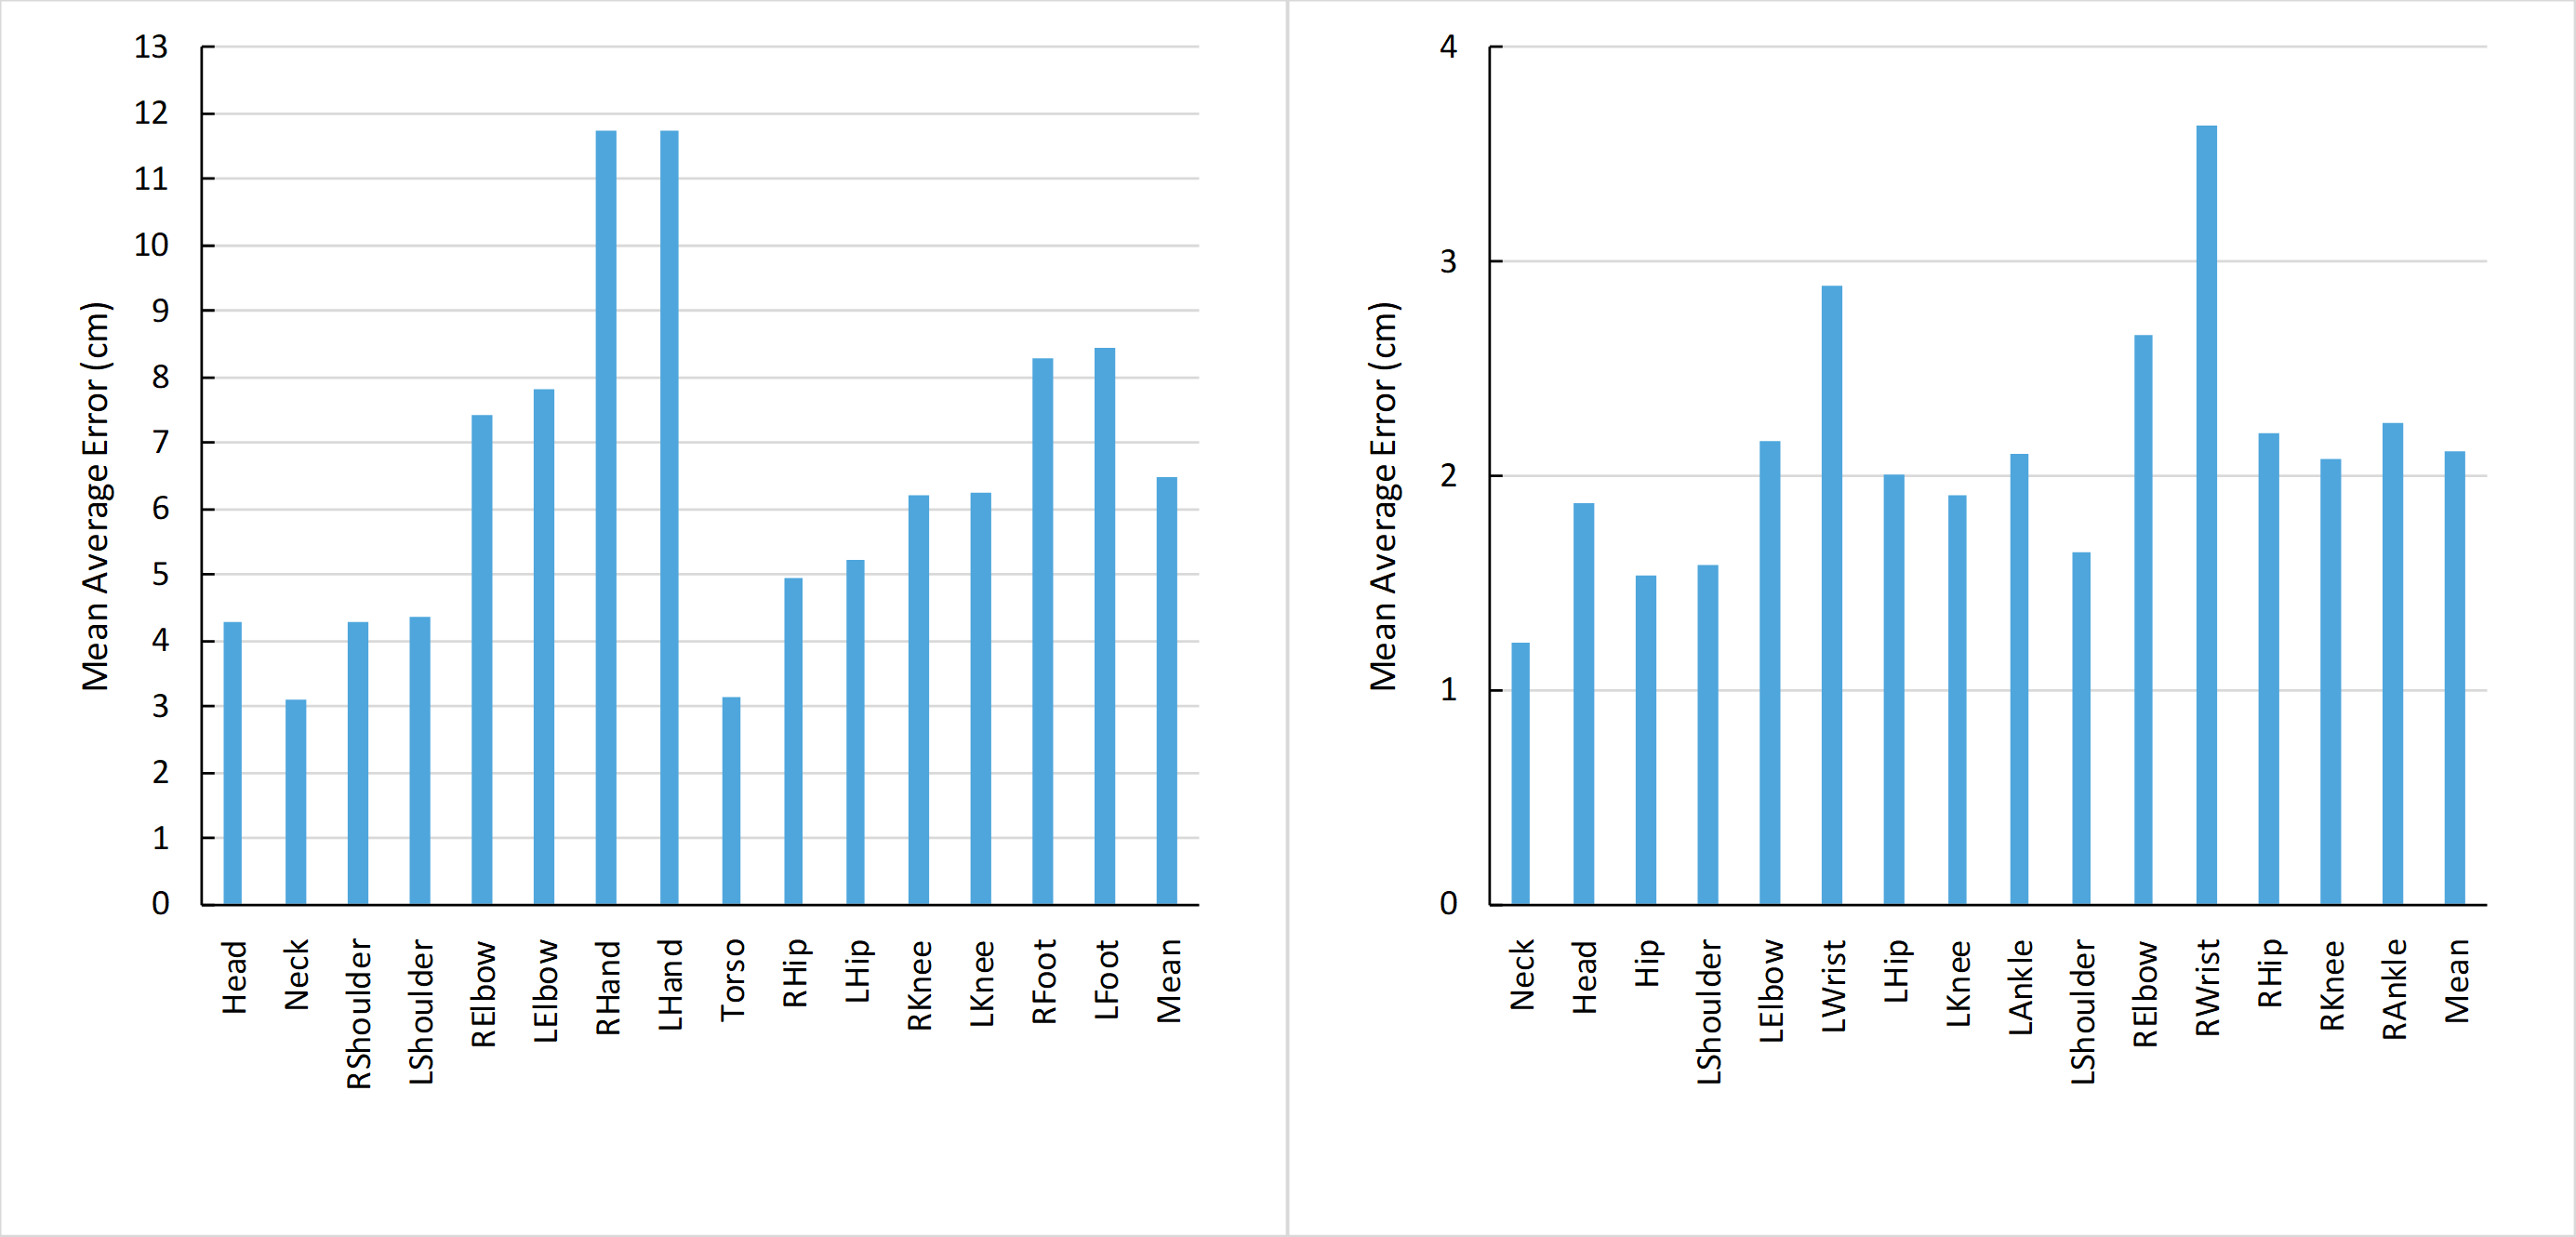
\includegraphics[width=\textwidth]{images/results/perjointerr2.png}
\caption[Mean average error per joint on ITOP and CMU dataset.]{Mean average error per joint on ITOP ({\it left}) and CMU ({\it right}) dataset.}
\label{fig:perjointerr2}
\end{center}
\end{figure}

\begin{figure}[H]
\begin{center}
\centering
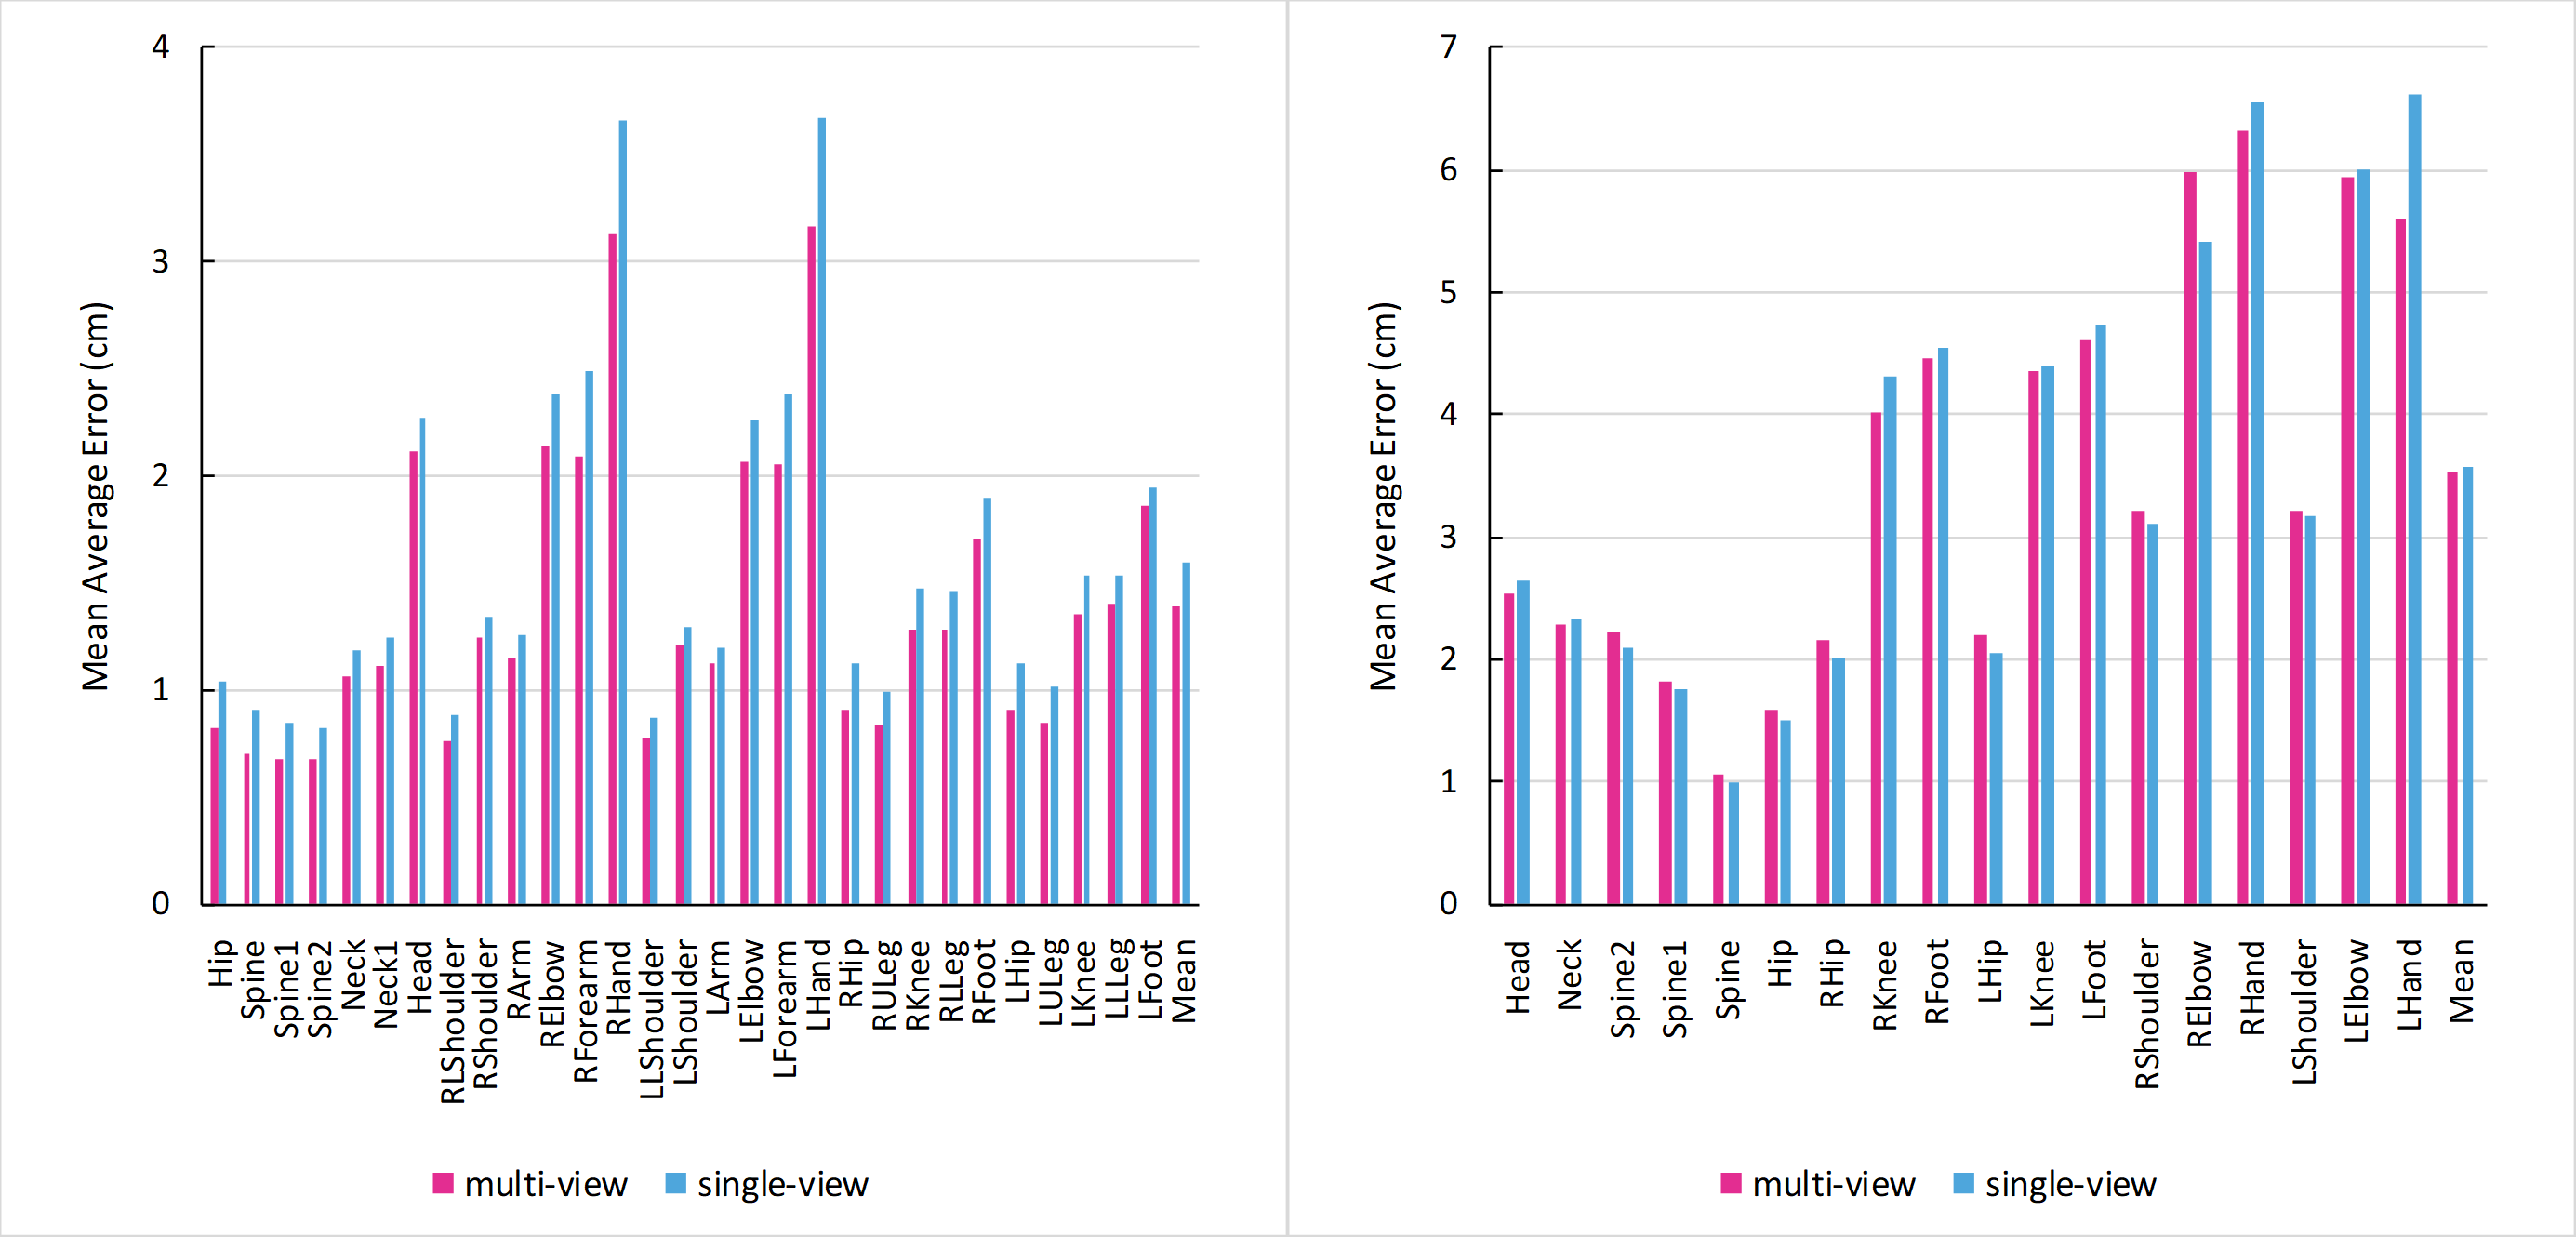
\includegraphics[width=\textwidth]{images/results/perjointerr1.png}
\caption[Mean average error per joint on MHAD and UBC3V dataset.]{Mean average error per joint on MHAD ({\it left}) and UBC3V ({\it right}) dataset, comparing multi-view and single-view approach.}
\label{fig:perjointerr1}
\end{center}
\end{figure}

\noindent
Regarding the CMU dataset, we evaluated our method specifically on the \textit{Range of motion} section of the dataset, yielding approximately 141K frames, as it was the only section capturing a single person, having ground truth labels available at the time of this research. Since prior to our work, there was no protocol established for the utilized section of the dataset, and considering the amount of data in the selected section of the dataset, we marked $20 \%$ of the data obtained by random sampling as the test set. There are also no existing results to compare to, concerning the single person pose estimation on this dataset (up to our knowledge). The mean per joint position error using our proposed approach is $2.11 \; \mbox{cm}$ (as shown in Figure~\ref{fig:perjointerr2}, right), and the mean average precision at $10 \; \mbox{cm}$ is  $98.39\%$. Figure~\ref{fig:cmu_results} illustrates the qualitative results on samples from CMU Panoptic dataset.\par
\vspace{5mm}

\begin{figure}[H]
\begin{center}
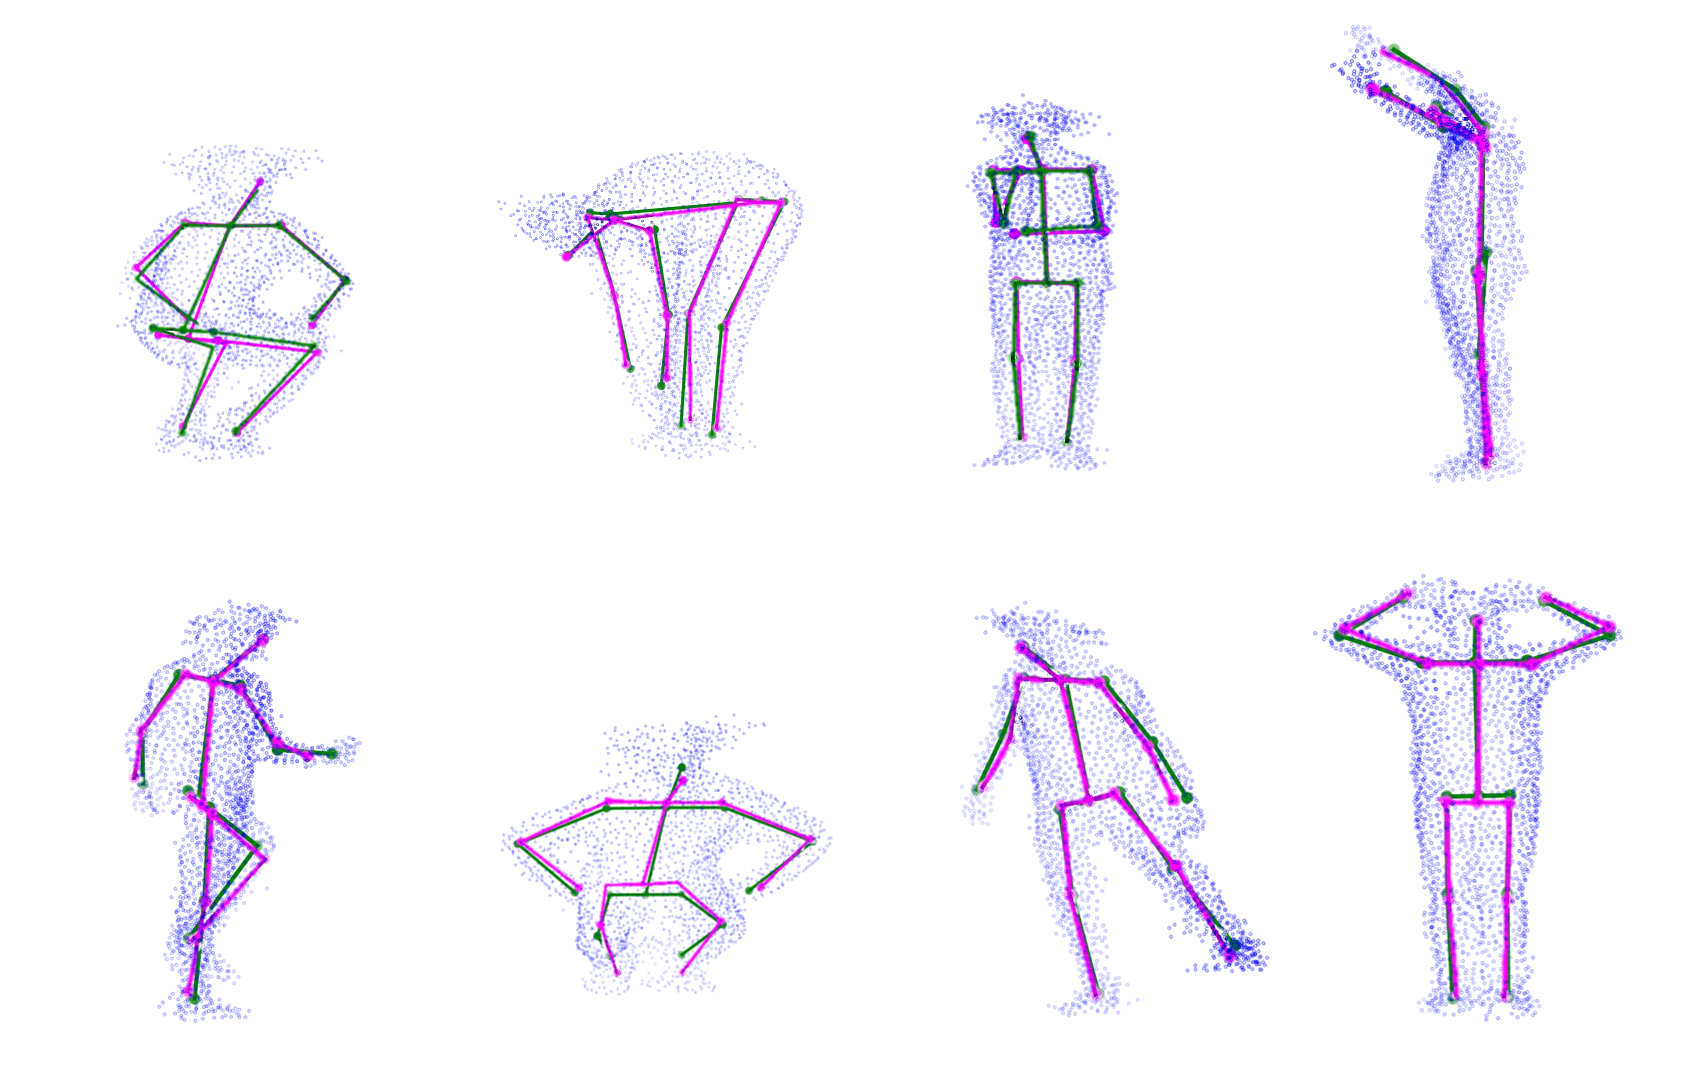
\includegraphics[height=190px]{images/results/CMU_results.png}
\caption[Qualitative results of our method on CMU Panoptic dataset.]{Qualitative results of our method on CMU Panoptic dataset. The ground truth skeletons ({\it green}) vs. our estimation ({\it magenta}). Best viewed in color.}
\label{fig:cmu_results}
\end{center}
\end{figure}

\noindent
Similarly, the MHAD dataset does not originally come with a train and test split, thus we carried out experiments using two different protocols: (a) choosing the test set as randomly sampled $25 \%$ of the dataset, (b) leave-one-subject-out cross validation. We present results of our approach on both the original full skeleton~(containing 35 joints) and the modified pruned skeleton~(29 joints) to be able to compare our strategy to the existing methods (as shown in Table~\ref{table:mhad_results}). Since in the case of the modified skeleton we have only removed redundant skeletal nodes, we have not reduced the complexity of the skeleton in a significant manner, but rather increased the focus on more relevant joints in the skeleton. As can be seen in Table~\ref{table:mhad_results}, the mean per joint position error has visibly decreased after omitting the redundant skeletal joints.\par
\vspace{5mm}

\setlength{\tabcolsep}{4pt}
\begin{table}[H]
\begin{center}
\caption[Mean per joint position error on MHAD dataset, compared to state-of-the-art methods.]{The mean per joint position error (MPJPE) of our approach on MHAD dataset evaluated following the leave-one-subject-out (LOSO) cross validation strategy, as well as randomly sampled test set, compared to state-of-the-art methods.}
\label{table:mhad_results}
\begin{tabular}{llll}
\hline\noalign{\smallskip}
Method & eval. protocol &MPJPE (cm) & MPJPE (cm) \\
& & single-view & multi-view\\
\noalign{\smallskip}
\hline
\noalign{\smallskip}
Shafei et. al~\cite{Shafaei16}& LOSO & – & 5.01\\ 
PBPE~\cite{Ali19} &random 25\%& 7.46 & 3.92\\
PBPE~\cite{Ali19} (29 joints)&random 25\% & 3.20 & –\\
\hline\noalign{\smallskip}
Ours - FCPE &LOSO& 3.97 &3.36 \\ 
Ours - FCPE  (29 joints)&LOSO& 3.23& 2.97\\ 
Ours - FCPE &random 25\%&  1.85  & 1.62\\ 
Ours - FCPE  (29 joints)&random 25\%& {\bf 1.59}& {\bf 1.39}\\ 
\hline
\end{tabular}
\end{center}
\end{table}
\setlength{\tabcolsep}{1.4pt}

\noindent It is important to point out that after the visual inspection of the MHAD dataset, the ground truth position labels in certain frames or sequences are noticeably shifted from the location of the corresponding skeletal joints, and clearly erroneous. Consequently, the model might overfit the training data, as in some cases the estimated joint position is visibly closer to the real joint location than the ground truth label.\par
\vspace{5mm}

\begin{figure}[H]
\begin{center}
\centering
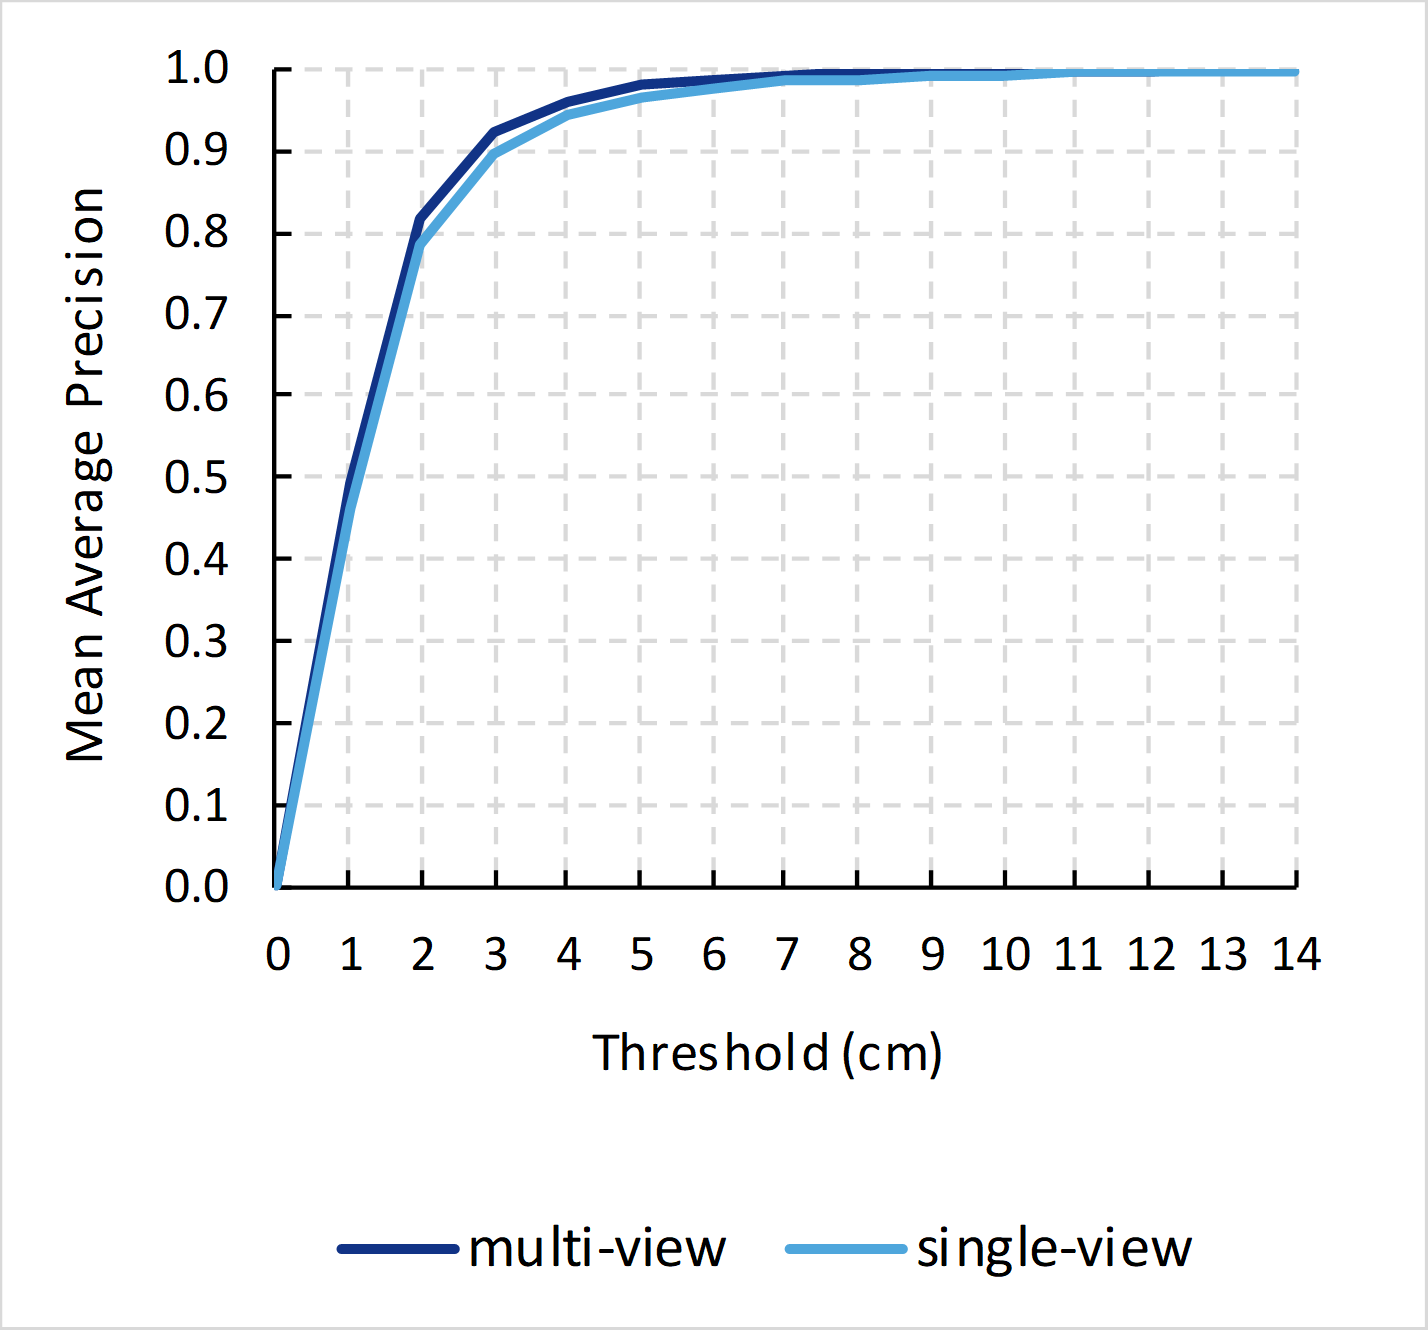
\includegraphics[height=170px]{images/results/MHAD_map.png}
\caption[Mean average precision at threshold on MHAD dataset.]{Mean average precision at threshold on MHAD dataset for multi-view and single-view approaches.}
\label{fig:MHAD_mAP}
\end{center}
\end{figure}


\noindent
Following the first protocol, i.e. establishing the test set as $25\%$ of the data by random sampling, our method achieves the mean per joint position error as low as $1.39\;\mbox{cm}$ for the multi-view approach, and $1.59\;\mbox{cm}$ for the single-view approach (as shown in Figure~\ref{fig:perjointerr1}, left), when using the modified skeleton structure. The achieved mean average precision at $10 \; \mbox{cm}$ is as high as $99.80 \; \%$ and $99.21 \; \%$ for the multi-view and single-view approach, respectively (Figure~\ref{fig:MHAD_mAP}). We set a novel state-of-the-art for MHAD dataset, lowering the mean per joint position error by  almost $65\%$ following the multi-view approach, and by approximately $50\%$ following the single-view approach.\par
\vspace{5mm}
\noindent
Table~\ref{table:UBC_results} summarizes the mean per joint position error on UBC3V hard-pose dataset for both single-view and multi-view approach. Using our approach, the achieved mean per joint position error is $3.57 \; \mbox{cm}$ in the case of single-view data, and $3.53 \; \mbox{cm}$ using multi-view data (as shown in Figure~\ref{fig:perjointerr1}, right). The mean average precision at $10 \; \mbox{cm}$ is $95.63 \; \%$ and $95.71 \; \%$ for the single-view and multi-view approach respectively. The claimed results of the Deep Depth Pose (DDP) model proposed in~\cite{Marin18jvcir} are listed in italics, due to a number of unsuccessful attemps to reproduce them by various researchers. The observed results on the reproduced DDP model, implemented following the same training procedures as the original implementation, are indicated in the table as well. Sample qualitative results on UBC3V hard-pose test set are shown in Figure~\ref{fig:ubc_results}, predicted on merged multi-view point clouds.\par
\vspace{5mm}

\setlength{\tabcolsep}{4pt}
\begin{table}[H]
\begin{center}
\caption[Mean per joint position error on UBC3V hard-pose dataset, compared to state-of-the-art methods.]{The mean per joint position error (MPJPE) of the proposed method on the test set of the UBC3V hard-pose dataset compared to state-of-the-art methods.}
\label{table:UBC_results}
\begin{tabular}{lll}
\hline\noalign{\smallskip}
Method & MPJPE (cm) & MPJPE (cm) \\
& single-view & multi-view\\
\noalign{\smallskip}
\hline
\noalign{\smallskip}
DDP (observed) &  19.23 & –\\
PBPE~\cite{Ali19} & 7.59 & 5.59\\
Shafei et. al~\cite{Shafaei16} & – & 5.64\\
DDP (claimed)~\cite{Marin18jvcir} & {\it 3.15} & {\it 2.36}\\
\hline\noalign{\smallskip}
Ours - FCPE & {\bf 3.57} & {\bf 3.53}\\
\hline
\end{tabular}
\end{center}
\end{table}
\setlength{\tabcolsep}{1.4pt}


\begin{figure}[H]
\begin{center}
\centering
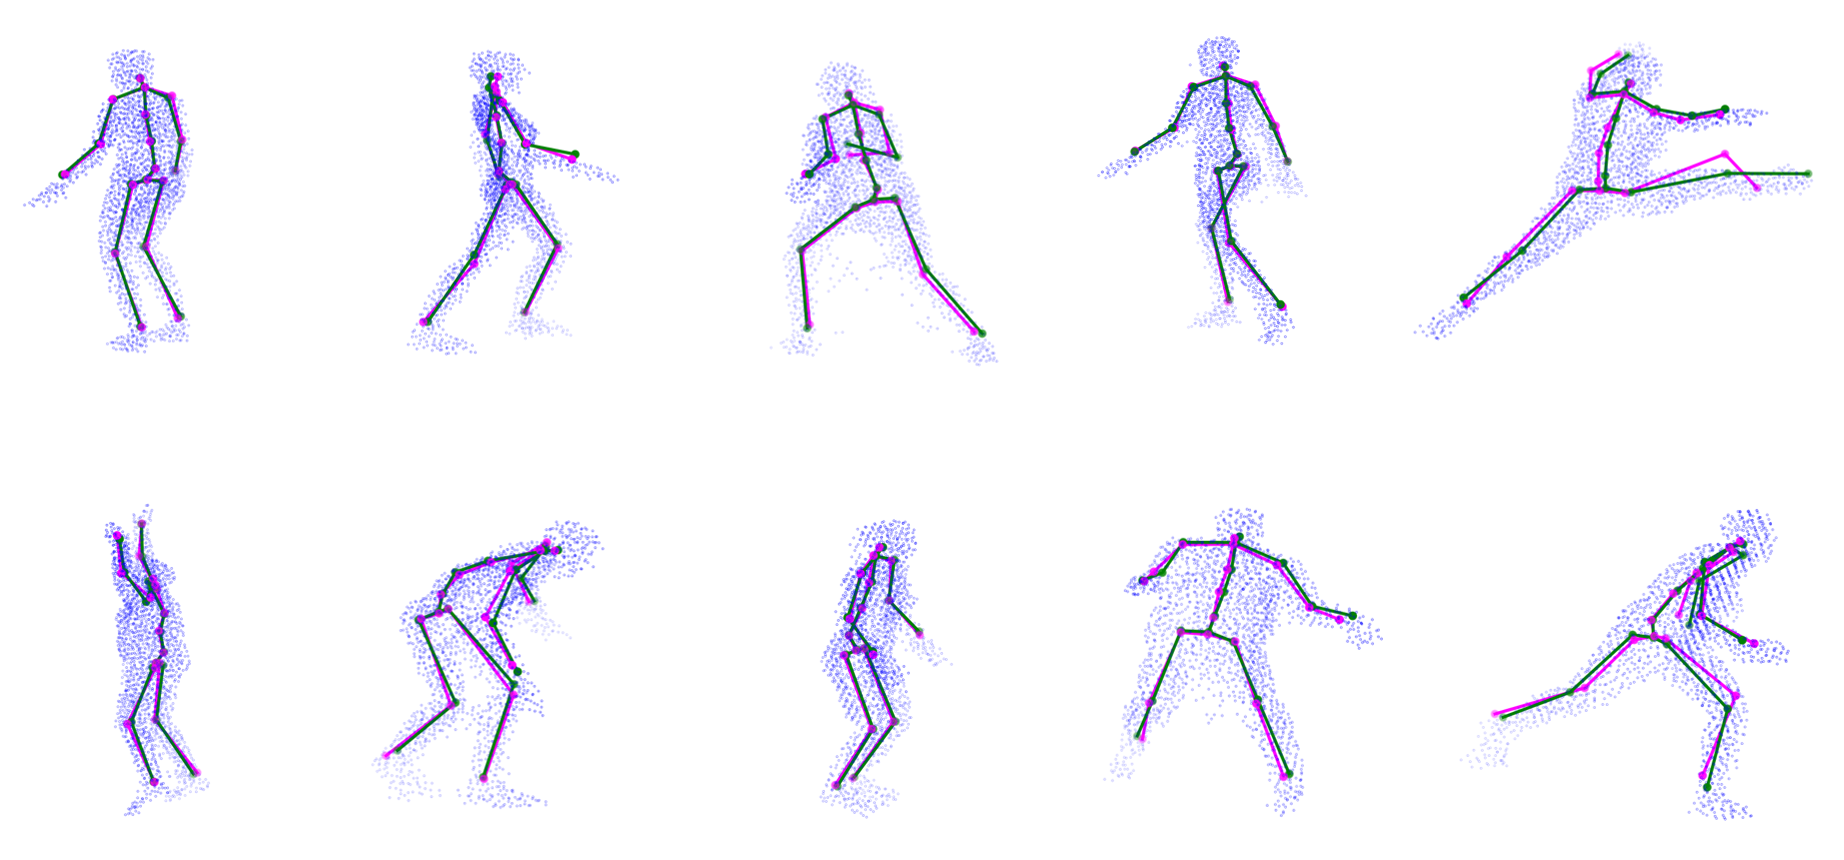
\includegraphics[height=140px]{images/results/UBC_results.png}
\caption[Qualitative results on test set of UBC hard-pose dataset.]{Qualitative results of our approach on test set of UBC hard-pose dataset. The ground truth skeletons ({\it green}) vs. our estimation ({\it magenta}). Best viewed in color.}
\label{fig:ubc_results}
\end{center}
\end{figure}

\noindent
We also present evaluation of the first stage of our pipeline. The accuracy of the semantic segmentation into the corresponding body regions over training epochs for all examined datasets is depicted in Figure~\ref{fig:seg_acc}. Our method achieves up to $95\%$ segmentation accuracy on CMU Panoptic dataset.\par
\vspace{5mm}

\begin{figure}[H]
\begin{center}
\centering
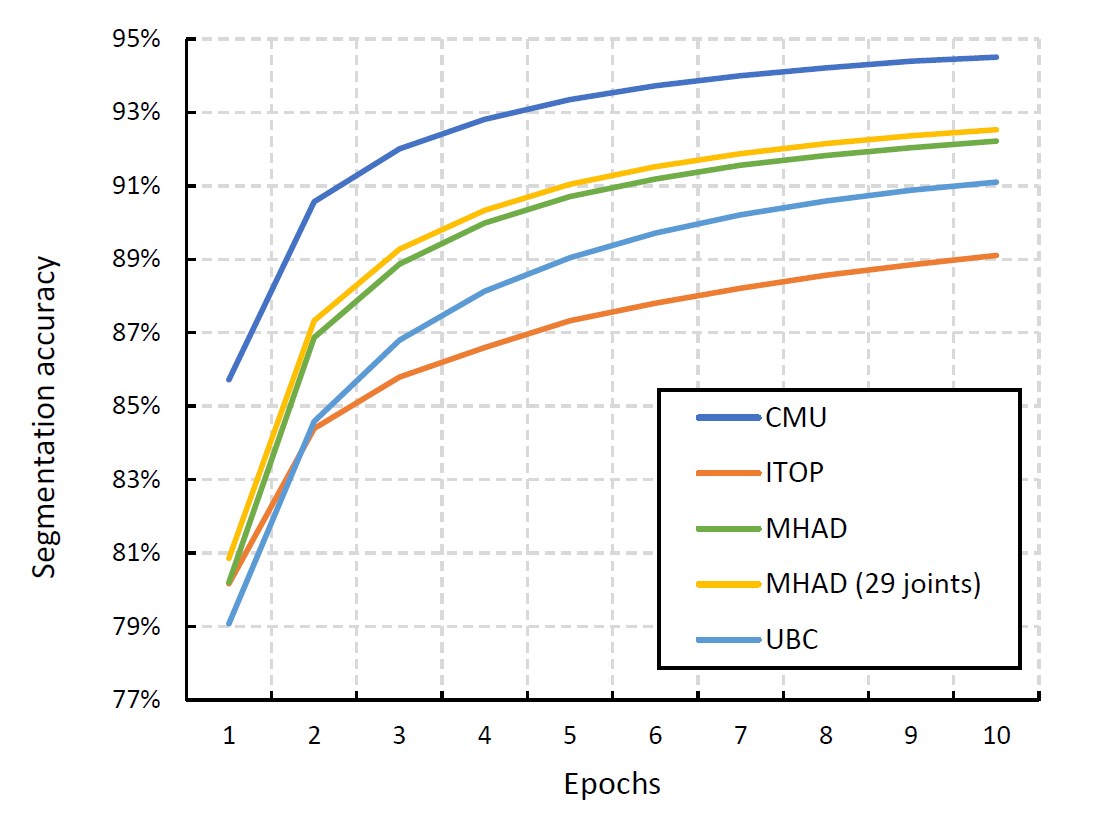
\includegraphics[height=180px]{images/results/segmentation_acc.png}
\caption[Accuracy of the body-parts segmentation of our method.]{Accuracy of the per-point body-parts segmentation performed in the first stage of our pipeline on all examined datasets.}
\label{fig:seg_acc}
\end{center}
\end{figure}
